% !TeX root = ../main.tex
% 中文精简审核稿：经作者确认后再同步 dp_puzzle.tex；当前中英文差异为有意保留。
\section{共享多精度点积微架构}
\label{sec:architecture}
\label{sec:brick_definition}

DP-Puzzle 采用 Lane、Group 和 DP（dot-product unit）三层结构（图~\ref{fig:dp_architecture}）。Lane 复用元素乘法与局部对齐，Group 融合尺度并统一部分和表示，DP 共享全局对齐与累加后端。统一的 Group 接口使低精度前端能够独立裁剪和增配，是后续配比扩展的组合边界。

H、Q、E 分别覆盖 FP16/BF16、MXFP8/6 和 MXFP4/NVFP4/HiF4，T、I 分别表示 TF32 和 INT8。一个 Lane 支持 T1H2I4Q4E8，数字表示每拍处理的元素对数。两个 Lane 构成 Group，四个 Group 构成 T8H16I32Q32E64 基线。该层级覆盖 HiF4 的局部微指数与 NVFP4 的组尺度粒度，更大尺度块通过广播共享尺度。各模式采用八级流水，每拍接收一笔独立请求。

\begin{figure}[t]
\centering
\includegraphics[width=\columnwidth]{baseline_arch.png}
\caption{Lane--Group--DP 分层架构。Lane 共享乘法与局部移位，Group 完成尺度融合与指数重计算，DP 共享全局对齐及累加；整数模式旁路浮点对齐与输出处理。}
\label{fig:dp_architecture}
\end{figure}

\subsection{Lane：解码与算术复用}
\label{sec:unpack_recode}
\label{sec:full_brick}

图~\ref{fig:data_unpack} 给出共享计算所需的解包表示：T/H 保留指数与有效数，Q 统一为内部 E5M3 表示，INT8 分离符号与幅值。MXFP4/NVFP4 将元素指数融入 U3P1 定点幅值；HiF4 将一级微指数并入 U2P2 幅值，保留 Lane 共享的二级微指数。E 类因此无需逐元素浮点对齐。

\begin{figure}[t]
\centering
% 图稿待作者统一数量标签：按完整 Lane 标注时，FP16 为 2x，E 为 8x；
% 右侧 10/16/4 位描述单个字段组，每个 Lane 包含两个字段组。
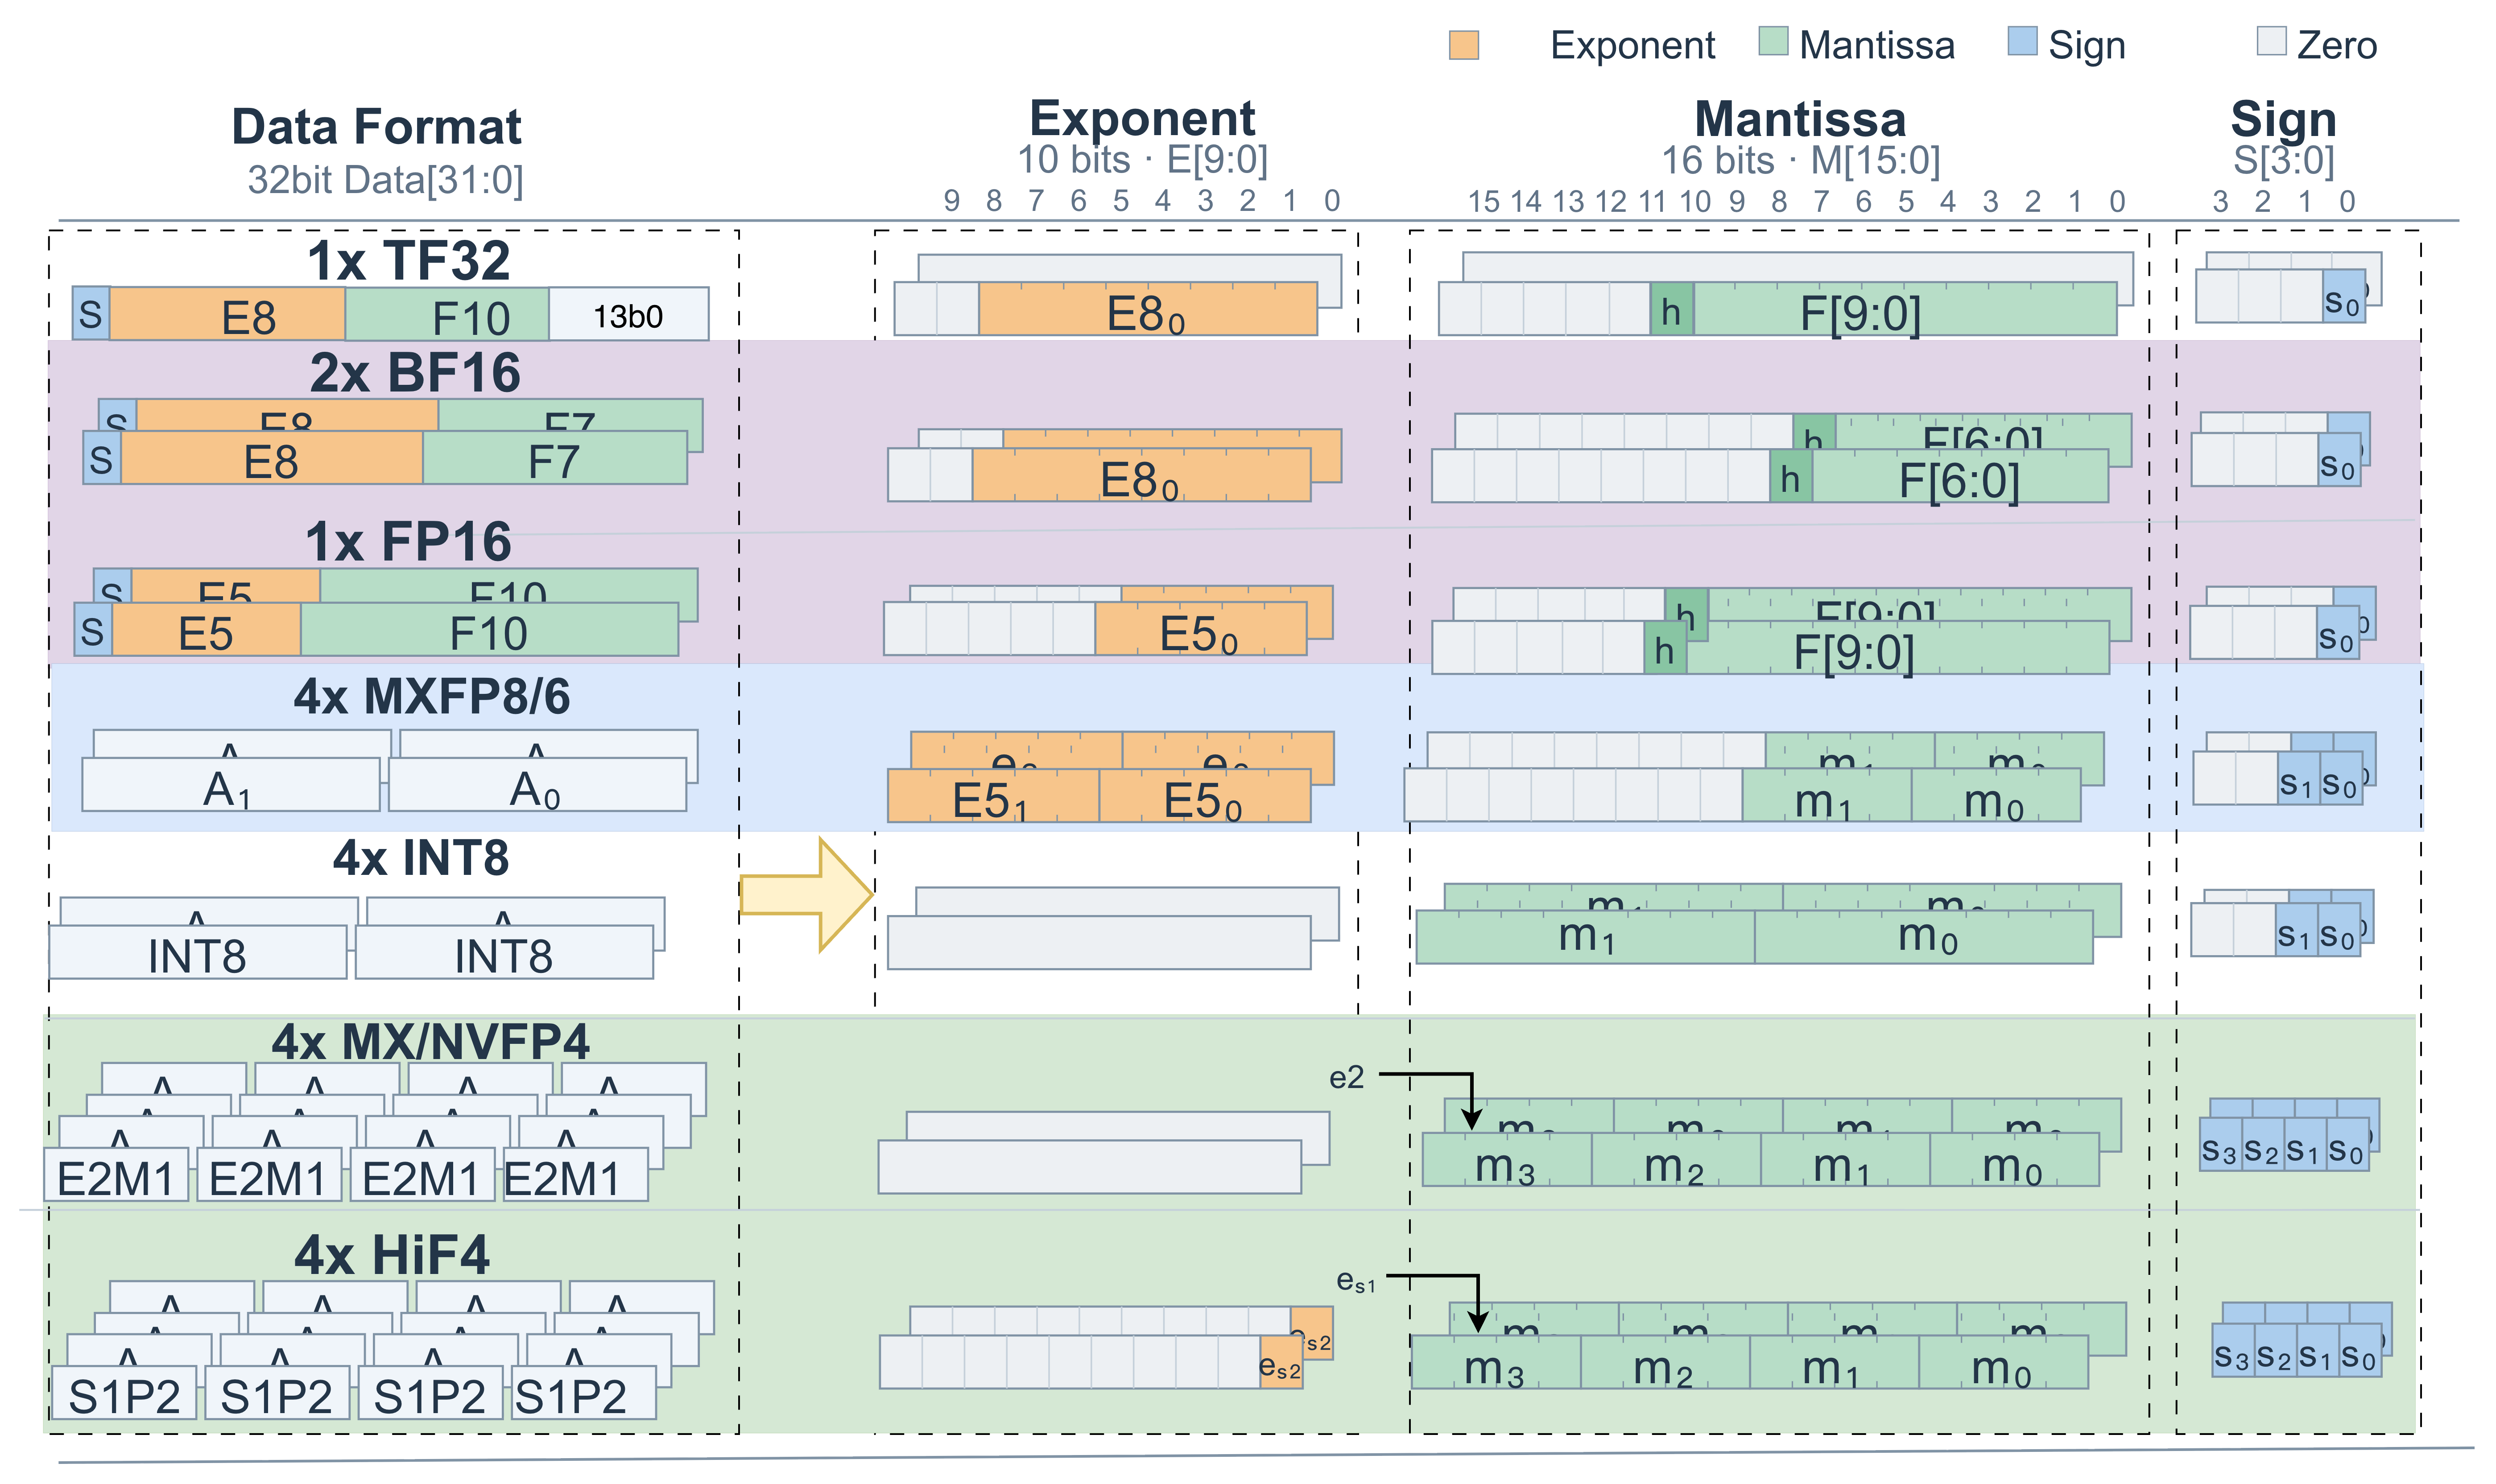
\includegraphics[width=\columnwidth]{unpack_layout.png}
\caption{输入格式到共享指数、有效数和符号字段的映射。Q 使用统一内部编码，E 将元素指数吸收到定点幅值中；未用字段补零，特殊值标志独立传播。}
\label{fig:data_unpack}
\end{figure}

\textbf{乘法器复用。}Ten-Four 按有效数位宽类别共享乘法器~\cite{rout2026tenfourv2}。本文采用两套 $8\times8$、$8\times4$、$4\times8$ 和 $4\times4$ 乘法单元，通过组合部分积支持宽乘法，通过独立路由支持多路低精度乘法，避免按格式复制完整乘法阵列。

\textbf{移位器复用。}T/H/Q 乘积按小数点位置静态补零后，进入四路共享右移器；本文选择 28\,bit 无符号局部对齐窗口。两个 Lane 使用共同的最大乘积指数完成对齐。E/INT8 旁路该网络，复用后续规约树；HiF4 在 Lane 部分和上施加二级微指数的小范围左移。

\subsection{Group：尺度融合与 Anchor Recompute}

\textbf{规约后尺度融合。}两个 Lane 共享尺度，Group 因而先求和并取幅值，再乘两侧尺度尾数的乘积 $\mathrm{Scale}_{\mathrm{mant}}$。NVFP4/HiF4 的紧凑组幅值为 U14，尺度尾数乘积为 U8，两种格式共用一套 U14$\times$U8 乘法器，避免逐元素复制尺度乘法。MX 的幂次尺度仅计入指数，旁路尾数乘法。

\textbf{统一部分和表示。}将 Group 输出幅值记为 $\mathrm{SoP}$（sum of products），位宽及小数位数分别记为 $\mathrm{Group}_{\mathrm{mag}}$ 和 $\mathrm{Group}_{\mathrm{frac}}$；本文采用 31\,bit 幅值。$\mathrm{Anchor}$ 表示幅值最高物理位对应的指数，由局部对齐指数 $\mathrm{Anchor}_{\mathrm{lane}}$、两侧尺度的无偏指数和 $\mathrm{Scale}_{\mathrm{exp}}$ 及元素偏置 $\mathrm{Bias}$ 共同确定：
\begin{equation}
\begin{aligned}
\mathrm{Anchor}={}&\mathrm{Anchor}_{\mathrm{lane}}+\mathrm{Scale}_{\mathrm{exp}}\\
 &+\mathrm{Group}_{\mathrm{mag}}-1-\mathrm{Group}_{\mathrm{frac}}-2\mathrm{Bias}.
\end{aligned}
\label{eq:anchor_recompute}
\end{equation}
格式相关修正可预先确定，使 Anchor Recompute 与尾数规约并行。E 的元素指数已融入幅值，局部对齐指数与元素偏置均取零；无尺度格式的尺度指数和取零。

\textbf{前导零与双向移位。}Group 在尺度融合后的 SoP 上检测前导零，以原始 Anchor 减去前导零数得到最高有效位的比较指数，零组不参与比较。原始 Anchor 同时保留，以其与全局最大比较指数之差控制双向移位，将规格化与全局对齐合并为一次操作。

\subsection{DP：共享累加与整数旁路}

各 Group 与 $C$ 在 39\,bit 无符号全局窗口内对齐，恢复符号后进入共享累加器。基线经 4:2 和 3:2 压缩及一次进位传播加法完成融合累加，输出端统一规格化与舍入。INT8/INT32 使用固定整数坐标，旁路浮点对齐及输出规格化舍入，复用累加通路。浮点幅值右移采用向零截断，最终 FP32 输出采用最近偶数舍入。
